% =====================================================================
% RESULTADOS – Consultas Q1 a Q4 y pregunta propia 1 (persona A)
% Archivo sections/04-results.tex. Requiere \usepackage{graphicx} en preamble.tex
% y los PDF en la carpeta figuras/ del proyecto de Overleaf.
% Números obtenidos de la base completa: 239.946 secuencias, 2.790 especies.
% =====================================================================

\subsection*{Composición de la base por clasificación (Q1)}

\textbf{Pregunta.} ¿Cuántos TEs hay por clase, por orden y por superfamilia?

\textbf{Resultado.} La Clase~I (retrotransposones) reúne 194\,774 secuencias
(81,2\,\%) y la Clase~II (transposones de ADN), 45\,172 (18,8\,\%). De los
11 órdenes, tres concentran el 93,4\,\% de la base: LTR (119\,368; 49,7\,\%),
LINE (68\,382; 28,5\,\%) y TIR (36\,471; 15,2\,\%). En el otro extremo,
PLE, RETROPOSON, CRYPTON y MAVERICK suman menos de 630 secuencias en
conjunto. Las 65 superfamilias tienen una distribución igualmente
desbalanceada: \textit{Copia} (21,2\,\%) y \textit{Gypsy} (18,3\,\%) cubren
casi el 40\,\% de la base, mientras que 16 superfamilias tienen menos de
100 secuencias.

\textbf{Interpretación.} La base está fuertemente sesgada hacia los
retrotransposones LTR. Para el diseño de la base de datos esto implica que
un índice sobre \texttt{te\_orden} es poco selectivo para los órdenes
mayoritarios: una consulta por LTR devuelve la mitad de la colección. Para
el uso de la base como insumo de clasificadores~\cite{orozcoarias2026panteon},
el desbalance indica que las clases minoritarias tendrán pocos ejemplos.
Además, 11 superfamilias tienen el mismo nombre que su orden (por ejemplo,
\texttt{LINE/LINE} o \texttt{TIR/TIR}; 21\,544 secuencias en total), lo que
en la práctica indica que la superfamilia no se determinó; estas secuencias
se conservaron, pero deben tratarse con cuidado en análisis por superfamilia.

% ---------------------------------------------------------------------
\subsection*{TEs por especie y clasificación (Q2)}

\textbf{Pregunta.} ¿Cuántos TEs tiene cada especie, desglosados por clase,
orden y superfamilia?

\textbf{Resultado.} La consulta produce 18\,513 combinaciones
especie--clasificación. La diversidad de superfamilias por especie es muy
variable: la mediana es de 5 superfamilias, pero \textit{Danio rerio}
alcanza 36 y 493 especies tienen una sola. Además, 652 especies tienen TEs
de un único orden. Por ejemplo, en \textit{Malus domestica}, la especie con
más TEs, predominan \textit{Copia} (671) y \textit{Gypsy} (398).

\textbf{Interpretación.} La mayoría de las especies tiene bibliotecas
pequeñas y poco diversas, sobre todo en Fungi, y unas pocas concentran
gran parte de las secuencias. Como la especie se guarda por referencia
(\texttt{especie\_id}), esta consulta exige un \texttt{\$lookup}; para
reducir su costo se agrupa primero en \texttt{secuencias} y luego se cruza
con \texttt{especies}, de modo que el \texttt{\$lookup} se ejecuta sobre
18\,513 grupos y no sobre 239\,946 documentos.

% ---------------------------------------------------------------------
\subsection*{Cambios entre reinos y phyla (Q3)}

\textbf{Pregunta.} ¿Cómo cambia la cantidad de TEs por clase y orden entre
reinos? ¿Y entre phyla?

\textbf{Resultado.} La composición difiere claramente entre reinos
(Figura~\ref{fig:composicion}). En Plantae, el 72,3\,\% de los TEs son LTR y
la Clase~I alcanza el 87,7\,\%. En Animalia predominan los LINE (44,0\,\%),
seguidos de LTR (25,1\,\%) y TIR (21,4\,\%). Fungi es intermedio, con LTR
(40,1\,\%) y LINE (31,0\,\%), y es el reino con mayor proporción de
HELITRON (8,6\,\%, frente a 1,2--1,9\,\% en los otros). RETROPOSON y CRYPTON
solo aparecen en Animalia. Por phyla, Angiosperma replica el patrón de
Plantae (73\,\% LTR), mientras que dentro de Animalia hay diferencias
marcadas: Arthropoda (61\,\%) y Mollusca (57\,\%) están dominados por LINE,
y Chordata está más repartido (LINE 35\,\%, LTR 29\,\%, TIR 25\,\%). En
Fungi, Basidiomycota y Mucoromycota tienen 13\,\% de HELITRON.

\begin{figure}[htbp]
  \centering
  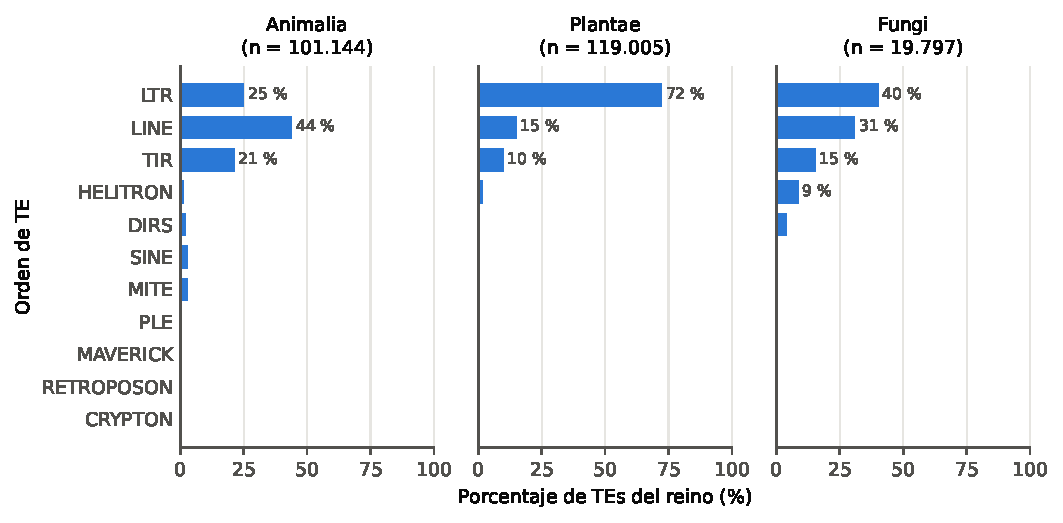
\includegraphics[width=\linewidth]{figuras/fig1_composicion_reino.pdf}
  \caption{Composición de TEs por reino: porcentaje de cada orden de TE
  dentro de Animalia, Plantae y Fungi (\textit{n} = número de TEs del
  reino). Datos obtenidos mediante agregación en MongoDB.}
  \label{fig:composicion}
\end{figure}

\textbf{Interpretación.} El predominio de LTR en plantas y de LINE en
animales es coherente con lo descrito para estos grupos. Sin embargo, estos
porcentajes describen las bibliotecas de PanTEon (familias de TEs
representadas en la base) y no la fracción del genoma que ocupa cada orden,
y el número de especies por reino es muy desigual (Fungi: 1\,559 especies
con una mediana de 5 TEs; Plantae: 451 especies con una mediana de 245).
Por eso se usan porcentajes dentro de cada reino en lugar de conteos
absolutos. La consulta depende de la taxonomía del CSV: cuatro secuencias
pertenecen a especies sin \textit{phylum} registrado.

% ---------------------------------------------------------------------
\subsection*{Longitud de los TEs por orden (Figura 2)}

\textbf{Resultado.} En toda la base, la longitud de los TEs va de 81 a
19\,926\,pb, con una mediana de 4\,259\,pb (Figura~\ref{fig:longitud}).
Los órdenes se separan en dos grupos. Los más cortos son SINE (mediana
254\,pb), CRYPTON (282\,pb) y MITE (346\,pb), cuyas cajas quedan por
debajo de 500\,pb. Los más largos son MAVERICK (6\,758\,pb), LTR
(5\,347\,pb; rango intercuartílico de 4\,314 a 6\,842\,pb) y DIRS
(5\,143\,pb). Entre ambos extremos están HELITRON (3\,371\,pb), LINE
(3\,279\,pb), PLE (2\,208\,pb), TIR (1\,341\,pb) y RETROPOSON (1\,159\,pb).
Varios órdenes muestran límites exactos: SINE y MITE no superan los
500\,pb, LINE va exactamente de 500 a 6\,000\,pb y TIR no llega a
10\,000\,pb, mientras que varios órdenes tienen un mínimo de 100\,pb.

\begin{figure}[htbp]
  \centering
  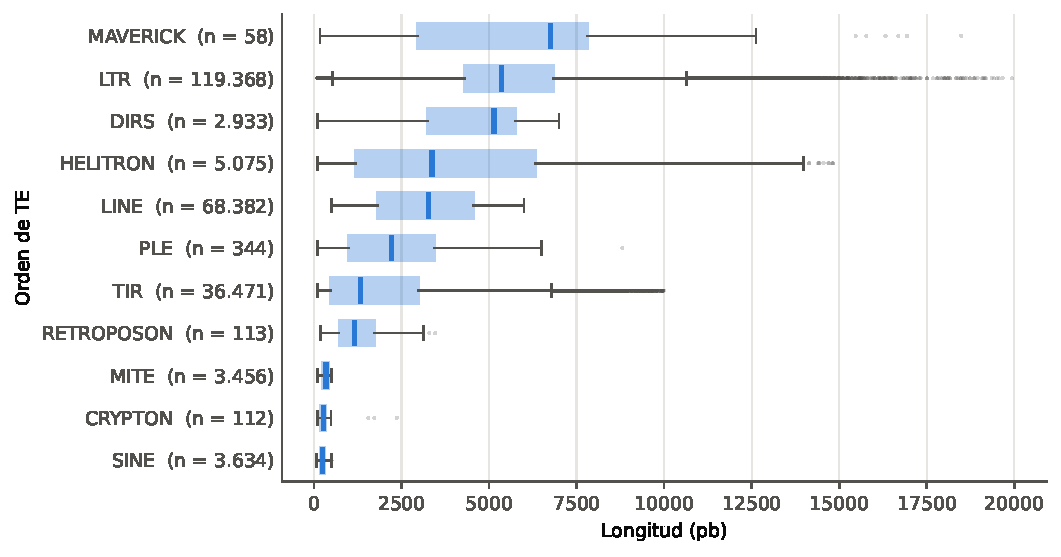
\includegraphics[width=\linewidth]{figuras/fig2_longitud_orden.pdf}
  \caption{Distribución de la longitud (pb) de los TEs por orden, ordenados
  por mediana; \textit{n} indica el número de secuencias de cada orden.
  Datos obtenidos de la colección \texttt{secuencias} en MongoDB.}
  \label{fig:longitud}
\end{figure}

\textbf{Interpretación.} La separación entre órdenes cortos y largos es
coherente con su estructura: los SINE y los MITE son elementos no
autónomos que no codifican las proteínas para movilizarse y por eso son
cortos, mientras que los LTR, DIRS y MAVERICK contienen genes completos y
superan con frecuencia los 5\,kb. Los cortes exactos (500, 6\,000 y
10\,000\,pb) no son biológicos: corresponden a los umbrales de longitud
por superfamilia que PanTEon aplicó al construir la base para conservar
solo secuencias con la estructura esperada~\cite{orozcoarias2026panteon}.
Por lo tanto, la Figura~\ref{fig:longitud} describe las secuencias
retenidas por esos filtros y no la longitud natural de cada orden. Un
caso que merece cautela es CRYPTON, cuya mediana (282\,pb) es mucho menor
de lo esperado para elementos que codifican una recombinasa, lo que
sugiere que muchas de sus 112 secuencias son fragmentos. Finalmente, la
amplia superposición entre órdenes como HELITRON, LINE y PLE muestra que
la longitud por sí sola no basta para clasificar un TE. Para la base de
datos, guardar \texttt{longitud} precalculada permite responder estas
consultas con una proyección de dos campos, sin leer las secuencias.

% ---------------------------------------------------------------------
\subsection*{Especies con más y menos TEs (Q4)}

\textbf{Pregunta.} ¿Cuáles son las 10 especies con más TEs y las 10 con menos?

\textbf{Resultado.} Encabezan la lista \textit{Malus domestica} (1\,627),
\textit{Danio rerio} (1\,352), \textit{Callithrix jacchus} (1\,294) y
Homininae (1\,173), seguidas de \textit{Nicotiana attenuata},
\textit{Colobus angolensis}, \textit{Chlorocebus sabaeus},
\textit{Geotrypetes seraphini}, \textit{Sitophilus oryzae} y
\textit{Oryza sativa} (1\,090). En el extremo opuesto, el mínimo es un
solo TE y lo comparten 326 especies.

\textbf{Interpretación.} Las 10 especies con menos TEs no están bien
definidas: con 326 empates en el mínimo, cualquier lista de diez es
arbitraria y depende del criterio de desempate (aquí, orden alfabético).
Es más informativo reportar cuántas especies tienen un solo TE. Por otro
lado, el cuarto lugar del top lo ocupa Homininae, que no es una especie
sino una subfamilia de primates; esto motivó la pregunta propia.

% ---------------------------------------------------------------------
\subsection*{Pregunta propia 1: ``especies'' que son taxones superiores}

\textbf{Pregunta.} ¿Cuántas entradas del campo especie corresponden en
realidad a taxones superiores, cuántos TEs aportan y de qué órdenes son?

\textbf{Resultado.} Se identificaron 45 entradas cuyo nombre tiene una
sola palabra (por ejemplo, Homininae, Myomorpha, Monotremata o Mammalia),
todas del reino Animalia. Aportan 3\,806 TEs (1,59\,\% de la base);
Homininae (1\,173) y Myomorpha (682) concentran casi la mitad. Por orden
predominan TIR (1\,920) y LTR (894).

\textbf{Interpretación.} Estas bibliotecas provienen de Dfam, donde las
familias se asignan a un nodo de la taxonomía (un clado) y no
necesariamente a una especie~\cite{storer2021dfam}. Por ello, el campo
\texttt{especie} no siempre contiene una especie, lo que afecta a las
consultas por especie (Q2 y Q4) y a la herencia de la taxonomía: estas
entradas no tienen niveles inferiores (por ejemplo, familia) bien definidos.
Se decidió conservarlas, porque eliminarlas haría perder 3\,806 secuencias
válidas, y documentarlas como una limitación del modelo.

% ---------------------------------------------------------------------
\subsection{Carga y validación de los datos}
La base de datos quedó organizada en tres colecciones relacionadas por
referencias: \texttt{especies} (2\,790 documentos), \texttt{secuencias}
(239\,946) y \texttt{kmers} (1\,439\,676, es decir, seis documentos por
secuencia, uno por cada $k=1,\dots,6$). Ninguna secuencia quedó sin
especie asociada. La carga de \texttt{especies} y \texttt{secuencias}
tardó 43{,}3\,s, y el cálculo e inserción de los \textit{k}-mers tardó
aproximadamente 1\,h\,10\,min con la versión secuencial del
\textit{pipeline}. El \textit{pipeline} es reanudable: una secuencia se
considera terminada cuando ya tiene su documento con $k=6$, y los
duplicados se rechazan mediante un índice único sobre
(\texttt{secuencia\_id}, \texttt{k}).
 
\paragraph{Estructura de los documentos de \textit{k}-mers.}
Cada documento de \texttt{kmers} contiene la referencia a la secuencia
(\texttt{secuencia\_id}), una copia de su orden (\texttt{te\_orden}), el
valor de $k$, el número de ventanas válidas (\texttt{total\_ventanas}) y
un diccionario \texttt{conteos} que guarda solo los \textit{k}-mers
presentes. Así, un 2-mer ausente no ocupa espacio y se interpreta como
frecuencia cero.
 
\paragraph{Tratamiento de caracteres no válidos.}
Toda ventana que contiene un carácter distinto de A, C, G o T se
descarta, y \texttt{total\_ventanas} cuenta solo las ventanas válidas,
de modo que las frecuencias (conteo/\texttt{total\_ventanas}) permanecen
normalizadas. Una sola N descarta $k$ ventanas para cada valor de $k$.
Las letras minúsculas se convierten a mayúsculas antes de contar.
 
% ---------------------------------------------------------------------
\subsection{Composición de la base por clasificación (Q1)}
 
\textbf{Pregunta.} ¿Cuántos TEs hay por clase, por orden y por superfamilia?
 
\textbf{Resultado.} La Clase~I (retrotransposones) reúne 194\,774 secuencias
(81,2\,\%) y la Clase~II (transposones de ADN), 45\,172 (18,8\,\%). De los
11 órdenes, tres concentran el 93,4\,\% de la base: LTR (119\,368; 49,7\,\%),
LINE (68\,382; 28,5\,\%) y TIR (36\,471; 15,2\,\%). En el otro extremo,
PLE, RETROPOSON, CRYPTON y MAVERICK suman menos de 630 secuencias en
conjunto. Las 65 superfamilias tienen una distribución igualmente
desbalanceada: \textit{Copia} (21,2\,\%) y \textit{Gypsy} (18,3\,\%) cubren
casi el 40\,\% de la base, mientras que 16 superfamilias tienen menos de
100 secuencias.
 
\textbf{Interpretación.} La base está fuertemente sesgada hacia los
retrotransposones LTR. Para el diseño de la base de datos esto implica que
un índice sobre \texttt{te\_orden} es poco selectivo para los órdenes
mayoritarios: una consulta por LTR devuelve la mitad de la colección. Para
el uso de la base como insumo de clasificadores~\cite{orozcoarias2026panteon},
el desbalance indica que las clases minoritarias tendrán pocos ejemplos.
Además, 11 superfamilias tienen el mismo nombre que su orden (por ejemplo,
\texttt{LINE/LINE} o \texttt{TIR/TIR}; 21\,544 secuencias en total), lo que
en la práctica indica que la superfamilia no se determinó; estas secuencias
se conservaron, pero deben tratarse con cuidado en análisis por superfamilia.
 
% ---------------------------------------------------------------------
\subsection{TEs por especie y clasificación (Q2)}
 
\textbf{Pregunta.} ¿Cuántos TEs tiene cada especie, desglosados por clase,
orden y superfamilia?
 
\textbf{Resultado.} La consulta produce 18\,513 combinaciones
especie--clasificación. La diversidad de superfamilias por especie es muy
variable: la mediana es de 5 superfamilias, pero \textit{Danio rerio}
alcanza 36 y 493 especies tienen una sola. Además, 652 especies tienen TEs
de un único orden. Por ejemplo, en \textit{Malus domestica}, la especie con
más TEs, predominan \textit{Copia} (671) y \textit{Gypsy} (398).
 
\textbf{Interpretación.} La mayoría de las especies tiene bibliotecas
pequeñas y poco diversas, sobre todo en Fungi, y unas pocas concentran
gran parte de las secuencias. Como la especie se guarda por referencia
(\texttt{especie\_id}), esta consulta exige un \texttt{\$lookup}; para
reducir su costo se agrupa primero en \texttt{secuencias} y luego se cruza
con \texttt{especies}, de modo que el \texttt{\$lookup} se ejecuta sobre
18\,513 grupos y no sobre 239\,946 documentos.
 
% ---------------------------------------------------------------------
\subsection{Cambios entre reinos y phyla (Q3)}
 
\textbf{Pregunta.} ¿Cómo cambia la cantidad de TEs por clase y orden entre
reinos? ¿Y entre phyla?
 
\textbf{Resultado.} La composición difiere claramente entre reinos
(Figura~\ref{fig:composicion}). En Plantae, el 72,3\,\% de los TEs son LTR y
la Clase~I alcanza el 87,7\,\%. En Animalia predominan los LINE (44,0\,\%),
seguidos de LTR (25,1\,\%) y TIR (21,4\,\%). Fungi es intermedio, con LTR
(40,1\,\%) y LINE (31,0\,\%), y es el reino con mayor proporción de
HELITRON (8,6\,\%, frente a 1,2--1,9\,\% en los otros). RETROPOSON y CRYPTON
solo aparecen en Animalia. Por phyla, Angiosperma replica el patrón de
Plantae (73\,\% LTR), mientras que dentro de Animalia hay diferencias
marcadas: Arthropoda (61\,\%) y Mollusca (57\,\%) están dominados por LINE,
y Chordata está más repartido (LINE 35\,\%, LTR 29\,\%, TIR 25\,\%). En
Fungi, Basidiomycota y Mucoromycota tienen 13\,\% de HELITRON.
 
\begin{figure}[htbp]
  \centering
  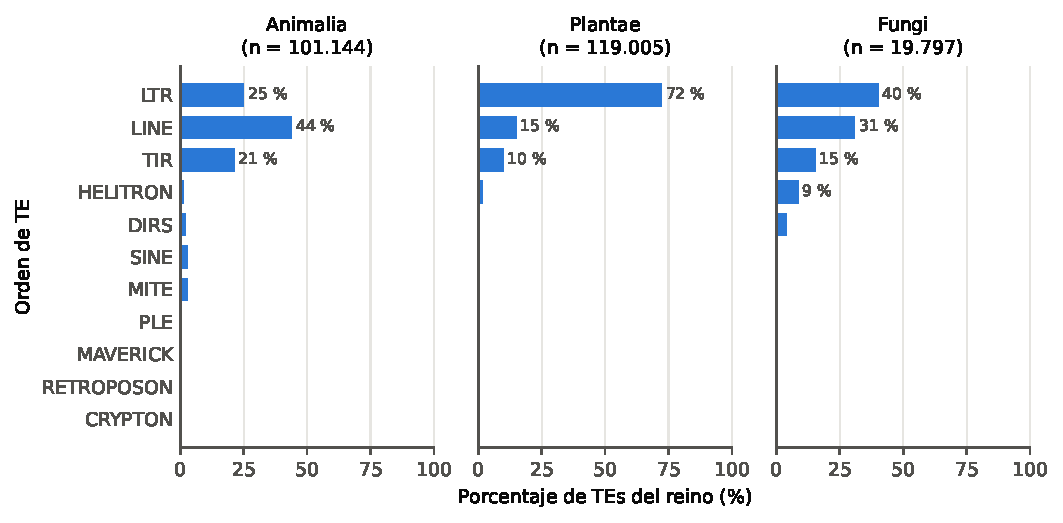
\includegraphics[width=\linewidth]{figuras/fig1_composicion_reino.pdf}
  \caption{Composición de TEs por reino: porcentaje de cada orden de TE
  dentro de Animalia, Plantae y Fungi (\textit{n} = número de TEs del
  reino). Datos obtenidos mediante agregación en MongoDB.}
  \label{fig:composicion}
\end{figure}
 
\textbf{Interpretación.} El predominio de LTR en plantas y de LINE en
animales es coherente con lo descrito para estos grupos. Sin embargo, estos
porcentajes describen las bibliotecas de PanTEon (familias de TEs
representadas en la base) y no la fracción del genoma que ocupa cada orden,
y el número de especies por reino es muy desigual (Fungi: 1\,559 especies
con una mediana de 5 TEs; Plantae: 451 especies con una mediana de 245).
Por eso se usan porcentajes dentro de cada reino en lugar de conteos
absolutos. La consulta depende de la taxonomía del CSV: cuatro secuencias
pertenecen a especies sin \textit{phylum} registrado.
 
% ---------------------------------------------------------------------
\subsection{Longitud de los TEs por orden}
 
\textbf{Resultado.} En toda la base, la longitud de los TEs va de 81 a
19\,926\,pb, con una mediana de 4\,259\,pb (Figura~\ref{fig:longitud}).
Los órdenes se separan en dos grupos. Los más cortos son SINE (mediana
254\,pb), CRYPTON (282\,pb) y MITE (346\,pb), cuyas cajas quedan por
debajo de 500\,pb. Los más largos son MAVERICK (6\,758\,pb), LTR
(5\,347\,pb; rango intercuartílico de 4\,314 a 6\,842\,pb) y DIRS
(5\,143\,pb). Entre ambos extremos están HELITRON (3\,371\,pb), LINE
(3\,279\,pb), PLE (2\,208\,pb), TIR (1\,341\,pb) y RETROPOSON (1\,159\,pb).
Varios órdenes muestran límites exactos: SINE y MITE no superan los
500\,pb, LINE va exactamente de 500 a 6\,000\,pb y TIR no llega a
10\,000\,pb, mientras que varios órdenes tienen un mínimo de 100\,pb.
 
\begin{figure}[htbp]
  \centering
  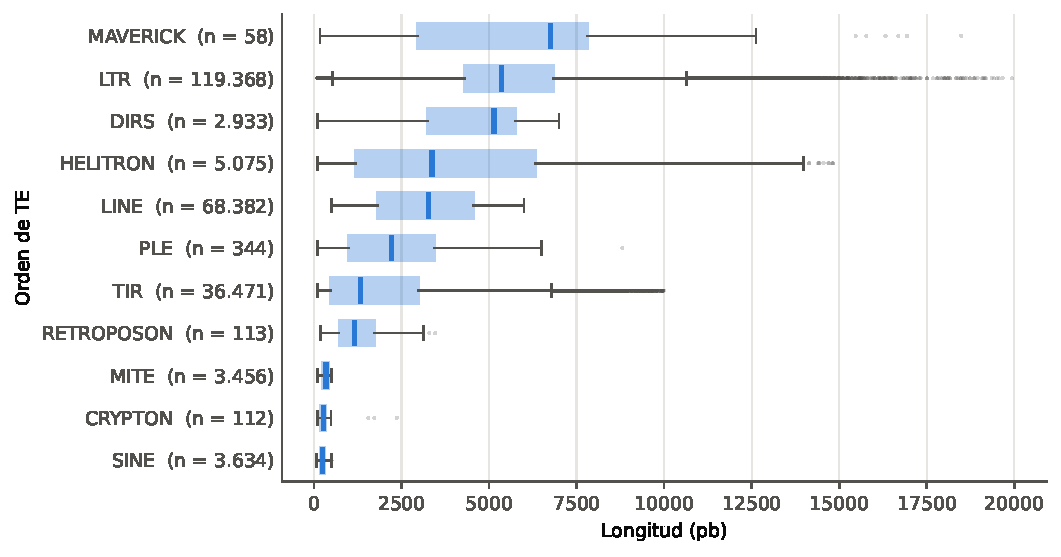
\includegraphics[width=\linewidth]{figuras/fig2_longitud_orden.pdf}
  \caption{Distribución de la longitud (pb) de los TEs por orden, ordenados
  por mediana; \textit{n} indica el número de secuencias de cada orden.
  Datos obtenidos de la colección \texttt{secuencias} en MongoDB.}
  \label{fig:longitud}
\end{figure}
 
\textbf{Interpretación.} La separación entre órdenes cortos y largos es
coherente con su estructura: los SINE y los MITE son elementos no
autónomos que no codifican las proteínas para movilizarse y por eso son
cortos, mientras que los LTR, DIRS y MAVERICK contienen genes completos y
superan con frecuencia los 5\,kb. Los cortes exactos (500, 6\,000 y
10\,000\,pb) no son biológicos: corresponden a los umbrales de longitud
por superfamilia que PanTEon aplicó al construir la base para conservar
solo secuencias con la estructura esperada~\cite{orozcoarias2026panteon}.
Por lo tanto, la Figura~\ref{fig:longitud} describe las secuencias
retenidas por esos filtros y no la longitud natural de cada orden. Un
caso que merece cautela es CRYPTON, cuya mediana (282\,pb) es mucho menor
de lo esperado para elementos que codifican una recombinasa, lo que
sugiere que muchas de sus 112 secuencias son fragmentos. Finalmente, la
amplia superposición entre órdenes como HELITRON, LINE y PLE muestra que
la longitud por sí sola no basta para clasificar un TE. Para la base de
datos, guardar \texttt{longitud} precalculada permite responder estas
consultas con una proyección de dos campos, sin leer las secuencias.
 
% ---------------------------------------------------------------------
\subsection{Especies con más y menos TEs (Q4)}
 
\textbf{Pregunta.} ¿Cuáles son las 10 especies con más TEs y las 10 con menos?
 
\textbf{Resultado.} Encabezan la lista \textit{Malus domestica} (1\,627),
\textit{Danio rerio} (1\,352), \textit{Callithrix jacchus} (1\,294) y
Homininae (1\,173), seguidas de \textit{Nicotiana attenuata},
\textit{Colobus angolensis}, \textit{Chlorocebus sabaeus},
\textit{Geotrypetes seraphini}, \textit{Sitophilus oryzae} y
\textit{Oryza sativa} (1\,090). En el extremo opuesto, el mínimo es un
solo TE y lo comparten 326 especies.
 
\textbf{Interpretación.} Las 10 especies con menos TEs no están bien
definidas: con 326 empates en el mínimo, cualquier lista de diez es
arbitraria y depende del criterio de desempate (aquí, orden alfabético).
Es más informativo reportar cuántas especies tienen un solo TE. Por otro
lado, el cuarto lugar del top lo ocupa Homininae, que no es una especie
sino una subfamilia de primates, lo que muestra que el campo de especie
también contiene taxones de rango superior.
 
% ---------------------------------------------------------------------
\subsection{Generación de bibliotecas (Q10 y Q11)}
 
\textbf{Pregunta.} ¿Cómo se obtiene, desde la base de datos y no desde el
archivo original, la biblioteca de una especie o de un reino dados?
 
\textbf{Resultado.} Una única función parametrizada por el nivel
taxonómico (\texttt{especie} o \texttt{reino}) y su valor consulta
primero \texttt{especies}, luego \texttt{secuencias} mediante el índice
de \texttt{especie\_id}, y escribe un archivo FASTA con el encabezado
original (\texttt{>ID\#CLASE/ORDEN/SUPERFAMILIA @Especie}) en la carpeta
\texttt{library/}. La biblioteca de \textit{Abortiporus biennis}
contiene 1 secuencia. La del reino Fungi contiene 1\,559 especies y
19\,797 secuencias, el 8{,}25\,\% de las 239\,946 de la base. El número
de especies coincide con el de Fungi obtenido en Q3.
 
\textbf{Interpretación.} Cambiar solo el parámetro basta para generar la
biblioteca de cualquier especie o reino sin leer el FASTA original. Esto
muestra que la referencia \texttt{especie\_id} permite construir
bibliotecas de cualquier nivel taxonómico con dos consultas indexadas.
El caso de \textit{A.\ biennis} también ilustra la cola de la
distribución descrita en Q4: hay especies con una sola secuencia.
 
% ---------------------------------------------------------------------
\subsection{Unión de secuencias con la taxonomía (Q12)}
 
\textbf{Pregunta.} ¿Cómo se recupera la taxonomía de la especie de cada TE?
 
\textbf{Resultado.} Una consulta con \texttt{\$lookup} sobre el campo
\texttt{especie\_id} devuelve, para cada TE, el reino, filo, clase, orden
y familia de su especie. Por ejemplo, la secuencia \texttt{PumCon-1.11}
(orden SINE) se une a \textit{Puma concolor}: Animalia, Chordata,
Mammalia, Carnivora, Felidae. Las secuencias \texttt{PDB00000001} y
\texttt{PDB00000002} (HELITRON) se unen a \textit{Halicephalobus
mephisto} (Animalia, Nematoda, Chromadorea, Rhabditida,
Panagrolaimidae).
 
\textbf{Interpretación.} Una sola referencia recupera toda la taxonomía,
que se almacena una vez en 2\,790 documentos y no se repite en las
239\,946 secuencias. Los identificadores no siguen todos el formato
\texttt{PDB\#\#\#\#\#\#\#\#} (existen identificadores como
\texttt{PumCon-1.11}), por lo que \texttt{pdb\_id} se trata como una
cadena arbitraria y única.
 
% ---------------------------------------------------------------------
\subsection{Comparación por origen de la biblioteca (Q13)}
 
\textbf{Pregunta.} Agrupando las especies según la columna \texttt{Source}
del CSV, ¿cuántas especies y secuencias hay en cada grupo, cuál es el
promedio de secuencias por especie y cuál la longitud promedio de los TEs?
 
\textbf{Resultado.} La Tabla~\ref{tab:origen} resume la comparación.
 
\begin{table}[htbp]
\centering
\caption{Comparación entre especies con biblioteca Dfam y RM2+MCH.}
\label{tab:origen}
\begin{tabular}{lrrrr}
\hline
Origen & Especies & Secuencias & Secuencias/especie & Longitud media (pb) \\
\hline
Dfam    & 386    & 31\,592  & 81{,}8 & 1\,653{,}8 \\
RM2+MCH & 2\,404 & 208\,354 & 86{,}7 & 4\,375{,}5 \\
\hline
\end{tabular}
\end{table}
 
Las especies con biblioteca RM2+MCH son el 86{,}2\,\% y aportan el
86{,}8\,\% de las secuencias. El número de secuencias por especie es
similar entre orígenes (86{,}7 frente a 81{,}8, una diferencia del
6\,\%), pero las secuencias de RM2+MCH son 2{,}6 veces más largas
(4\,375 frente a 1\,654\,pb).
 
\textbf{Interpretación.} Los dos orígenes no son equivalentes en
longitud, y cualquier análisis que compare especies de ambos grupos debe
tenerlo en cuenta. La causa no se midió: puede deberse a la composición
de órdenes de cada grupo (los órdenes largos y cortos difieren mucho en
longitud, según la sección anterior) o a la forma de construir cada
biblioteca. La longitud media es un promedio ponderado por secuencia.
 
% ---------------------------------------------------------------------
\subsection{Control de calidad (Q14)}
 
\textbf{Pregunta.} ¿Cuántas secuencias contienen caracteres distintos de
A, C, G y T, y cuántas posiciones se descartan por ello?
 
\textbf{Resultado.} La consulta encontró 54\,837 secuencias (22{,}85\,\%)
con caracteres distintos de A, C, G o T. Todas tenían
\texttt{porcentaje\_n}\,>\,0, de modo que ese campo detecta todas las
secuencias afectadas. Se descartaron 2\,147\,161 posiciones, el
0{,}223\,\% de las 963\,901\,415 bases, unas 39 por secuencia afectada.
 
\textbf{Interpretación.} Casi una de cada cuatro secuencias tiene al
menos un carácter ambiguo, pero la pérdida de información es mínima.
Descartar solo las ventanas afectadas, y no secuencias enteras, evita
eliminar 54\,837 TEs. La política queda justificada, y las frecuencias
siguen normalizadas por \texttt{total\_ventanas}. El control no distingue
si los caracteres no válidos son siempre N o incluyen otros códigos IUPAC.
 
% ---------------------------------------------------------------------
\subsection{Perfil de \textit{k}-mers de una secuencia (Q15)}
 
\textbf{Pregunta.} ¿Cuál es el perfil de \textit{k}-mers de una secuencia
dada para un $k$ dado?
 
\textbf{Resultado.} La función recibe el identificador de la secuencia y
$k$, busca la secuencia por \texttt{pdb\_id} (índice único) y recupera su
documento por (\texttt{secuencia\_id}, \texttt{k}), también indexado. Para
\texttt{PDB00000001} (GC\,=\,31{,}5\,\%) con $k=3$ hay 1\,989 ventanas
válidas. Los diez 3-mers más frecuentes suman 771 ventanas, el
38{,}8\,\% del total. Ocho de ellos están formados solo por A y T (AAA,
TTT, AAT, ATT, TAT, ATA, TAA y TTA) y los otros dos (GAA y ATG)
contienen una sola G. El más frecuente, AAA, representa el 7{,}2\,\% de
las ventanas, frente al 4{,}9\,\% de TTT.
 
\textbf{Interpretación.} El perfil es coherente con el bajo contenido de
GC de la secuencia, lo que indica que los conteos almacenados reproducen
su composición. Con una sola secuencia no es posible generalizar la
asimetría entre AAA y TTT.
 
% ---------------------------------------------------------------------
\subsection{Perfiles de dinucleótidos por orden de TE}
 
\textbf{Pregunta.} ¿Hay órdenes de TE con perfiles de 2-mers parecidos o
muy distintos?
 
\textbf{Resultado.} La Figura~\ref{fig:heatmap} muestra la frecuencia
promedio de los 16 dinucleótidos en cada uno de los 11 órdenes. El
promedio se calcula sobre la frecuencia de cada secuencia, de modo que
una secuencia larga no pesa más que una corta; las 16 frecuencias de
cada orden suman 1. Los órdenes más parecidos, medidos por distancia
euclidiana entre perfiles, son HELITRON--TIR (0{,}0151), MITE--TIR
(0{,}0159) y LINE--LTR (0{,}0168). Los más distintos son MAVERICK--SINE
(0{,}1076), HELITRON--SINE (0{,}0977) y SINE--TIR (0{,}0975). SINE
aparece en cuatro de los cinco pares más alejados: tiene TT bajo
(0{,}048 frente a 0{,}082--0{,}104 en HELITRON, LINE, LTR, MAVERICK, MITE
y TIR), AT bajo (0{,}042), y GG y CC altos (0{,}090 y 0{,}076). La
separación entre extremos es unas siete veces la distancia entre los
órdenes más parecidos. CG es el dinucleótido menos frecuente en casi
todos los órdenes, con un mínimo de 0{,}030 en LINE y LTR.
 
\begin{figure}[htbp]
\centering
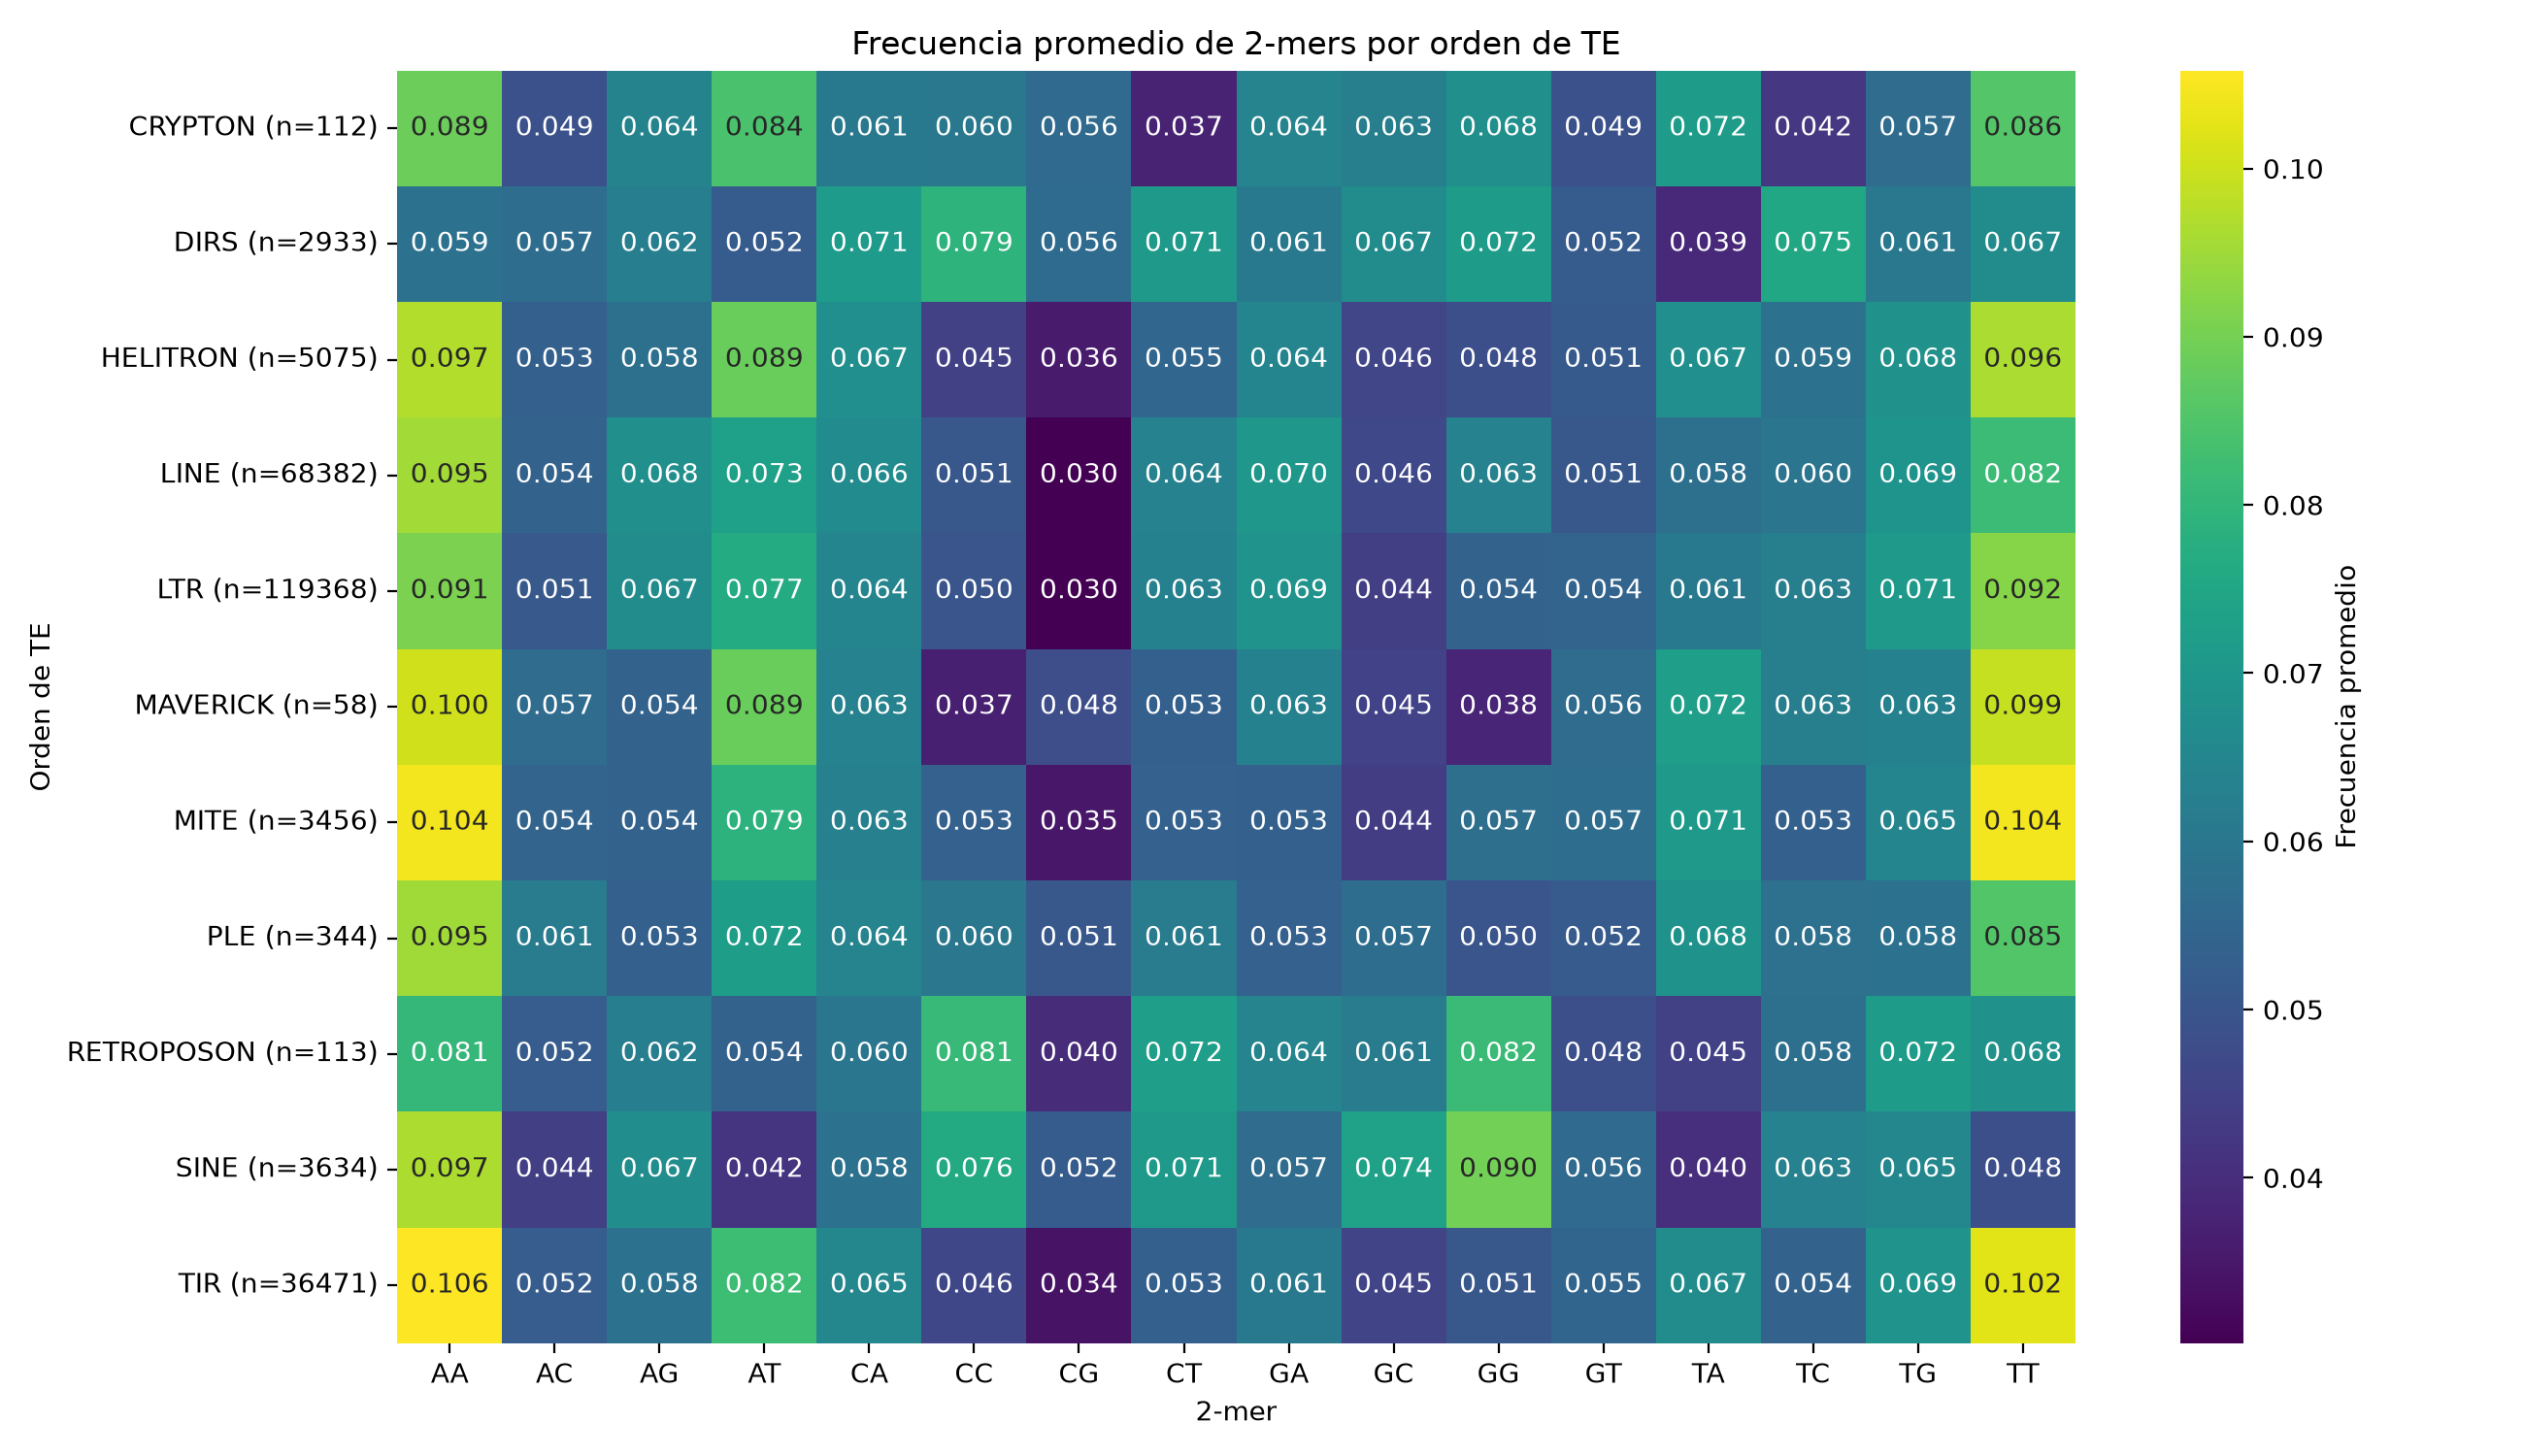
\includegraphics[width=\linewidth]{figuras/heatmap_2mers_orden.png}
\caption{Frecuencia promedio de los 16 2-mers por orden de TE
(promedio de las frecuencias por secuencia; \textit{n} es el número de
secuencias del orden).}
\label{fig:heatmap}
\end{figure}
 
\begin{figure}[htbp]
\centering
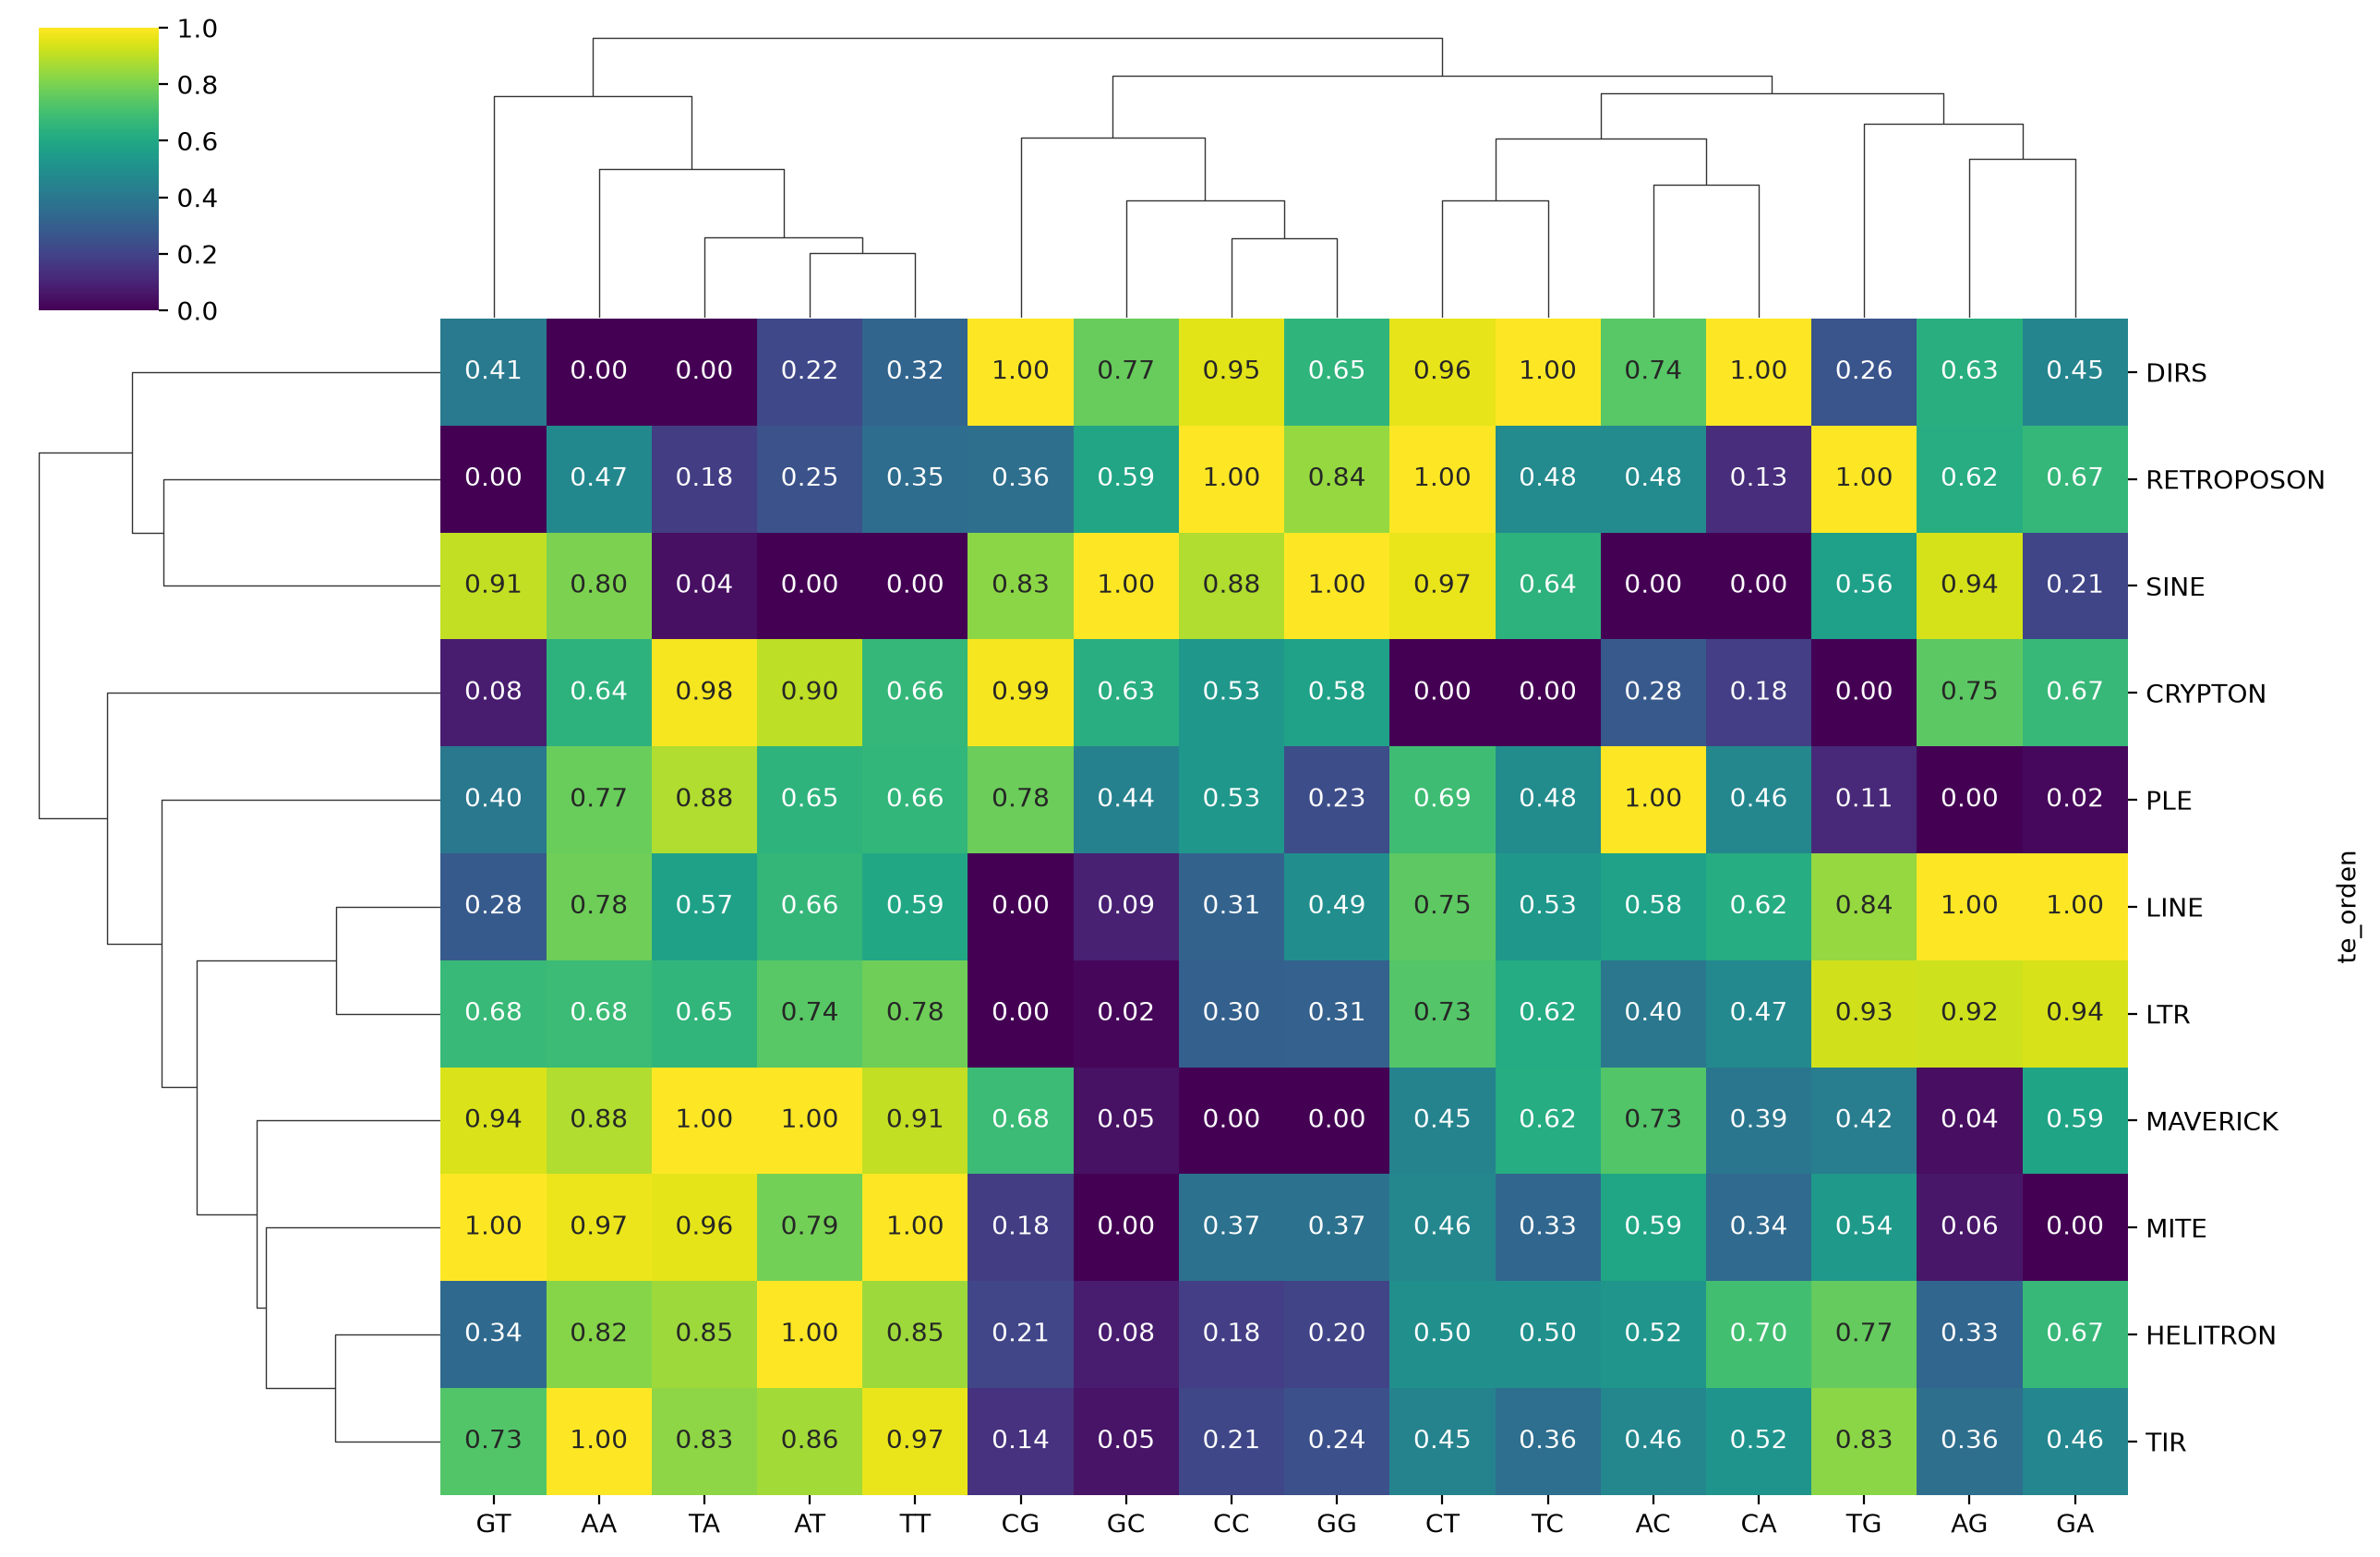
\includegraphics[width=\linewidth]{figuras/clustermap_2mers_orden.png}
\caption{Agrupamiento jerárquico de los órdenes. Los valores están
reescalados por columna (0 a 1), por lo que los extremos 0 y 1 no son
frecuencias reales; las frecuencias reales están en la
Figura~\ref{fig:heatmap}.}
\label{fig:cluster}
\end{figure}
 
\textbf{Interpretación.} Los perfiles de 2-mers distinguen órdenes: TIR,
MITE, HELITRON y MAVERICK comparten AA y TT altos y CG bajo, LINE y LTR
forman otro par muy parecido, y SINE se aparta del resto. El número de
secuencias por orden es muy desigual (de 58 en MAVERICK a 119\,368 en
LTR), por lo que los promedios de MAVERICK, CRYPTON ($n=112$) y
RETROPOSON ($n=113$) son menos fiables que los de LTR, LINE o TIR.